%%%%%%%%%%%%%%%%%%%%%%%%%%%%%%%%%%%%%%%%%
% Structured General Purpose Assignment
% LaTeX Template
%
% This template has been downloaded from:
% http://www.latextemplates.com
%
% Original author:
% Ted Pavlic (http://www.tedpavlic.com)
%
% Note:
% The \lipsum[#] commands throughout this template generate dummy text
% to fill the template out. These commands should all be removed when 
% writing assignment content.
%
%%%%%%%%%%%%%%%%%%%%%%%%%%%%%%%%%%%%%%%%%

\documentclass{article}

\usepackage{fancyhdr} % Required for custom headers
\usepackage{lastpage} % Required to determine the last page for the footer
\usepackage{extramarks} % Required for headers and footers
\usepackage{graphicx} % Required to insert images
\usepackage[utf8]{inputenc}

% Margins
\topmargin=-0.45in
\evensidemargin=0in
\oddsidemargin=0in
\textwidth=6.5in
\textheight=9.0in
\headsep=0.25in 

\linespread{1.1} % Line spacing



\setlength\parindent{0pt} % Removes all indentation from paragraphs

%----------------------------------------------------------------------------------------
%	DOCUMENT STRUCTURE COMMANDS
%	Skip this unless you know what you're doing
%----------------------------------------------------------------------------------------

% Header and footer for when a page split occurs within a problem environment
\newcommand{\enterProblemHeader}[1]{
\nobreak\extramarks{#1}{#1 continued on next page\ldots}\nobreak
\nobreak\extramarks{#1 (continued)}{#1 continued on next page\ldots}\nobreak
}

% Header and footer for when a page split occurs between problem environments
\newcommand{\exitProblemHeader}[1]{
\nobreak\extramarks{#1 (continued)}{#1 continued on next page\ldots}\nobreak
\nobreak\extramarks{#1}{}\nobreak
}

\setcounter{secnumdepth}{0} % Removes default section numbers
\newcounter{homeworkProblemCounter} % Creates a counter to keep track of the number of problems

%----------------------------------------------------------------------------------------
%	NAME AND CLASS SECTION
%----------------------------------------------------------------------------------------

\newcommand{\lessonNumber}[1]{Lezione\ \##1} % Assignment title
\newcommand{\lessonDate}[4]{#1,\ #2\ #3\ #4} % Due date
\newcommand{\lessonCourse}[1]{#1} % Course/class
\newcommand{\lessonTime}[1]{#1} % Class/lecture time
\newcommand{\lessonTeacher}[1]{#1} % Teacher/lecturer
\newcommand{\lessonAuthor}[1]{#1} % Your name
\begin{document}

\section{Considerazioni strategiche(11)}

Il segmento di ciclo di vita attivato nel progetto didattico va dalla RR \textit{Revisione dei Requisiti} alla RA \textit{Revisione Accettazione}.

Per il committente non è positivo avere un modello sequenziale, perché non avrà  mai visione del prodotto se non alla fine, non riceve prototipi e quindi perde interesse nel progetto, e noi vogliamo un proponente che sia \textbf{attivo} e interessato al nostro prodotto. Una volta acquisita l'esperienza necessaria allora posso usare un modello un po' più agile. Il \textbf{modello di sviluppo interno} serve a noi per trovare il miglior compromesso tra esigenze diverse. E' una scelta autonoma del fornitore e determina il piano strategico di utilizzo delle risorse disponibili (persone, capacità , strumenti).\\

Ciascuno di noi deve formare un gruppo portando un proprio \textbf{calendario} già  fatto, fissando dei vincoli e delle previsioni strategiche. Bisogna far emergere una disciplina ed avere alcune accortezze. Si parla dunque di \textbf{pianficazione}. Un \textit{mese-persona} vale circa 142 ore. Il modo in cui gestisco tempo e persone è molto delicato:

\begin{itemize}

	\item Vi sono componenti di impegno \textbf{non comprimibili}, ovvero non posso mettere più persone sullo stesso compito, non posso svolgerlo in parallelo. Non posso frantumare in piccole parti da parallelizzare (es. programmazione o verifica). Le cose sulle quali riesco a comprimere sono poche;
	\item Vi sono compiti \textbf{non partizionabili};
	\item La verifica a livello di sistema si fa \textbf{solo alla fine}, perché non sono test parallelizzabili e il sistema diventa disponibile solo alla fine dello sviluppo.

\end{itemize}

Occorre avere una pianificazione che abbia margini e che sia completamente consapevole dei vincoli. Una buona progettazione consente di non cadere nella iterazione non controllata. In questo modo, con queste tecniche si migliora la \textit{mitigazione dei rischi}.\\
Che tipo di modello di ciclo di vita devo scegliere? Dobbiamo scegliere una strategia che sia buona per noi. Il modello sequenziale è esattamente coerente con quello che si aspetta il committente, ma non per quanto riguarda il proponente.

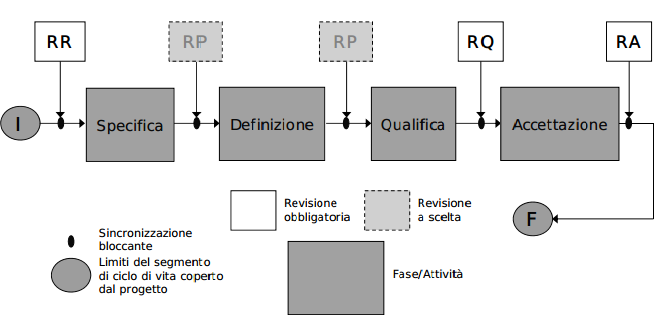
\includegraphics[width=0.5\columnwidth]{img1}

Il \textbf{modello incrementale} non è iterativo, l'iterazione \textit{distrugge} per sostituzione, potenzialmente pericolosa. La posso avere solo in situazioni di emergenza. Un ciclo incrementale può essere visto come un "\textit{for}". Ogni passaggio di questo ciclo aggiunge cose, mi avvicino alla soluzione per approssimazioni non distruttive, quindi additive. Posso anche non incrementare ma l'importante è che il numero di iterazioni sia noto. Dentro una chiamata di RP posso portare più di un incremento, tuttavia il progetto didattico prevede una singola occorrenza di ogni revisione. Il fornitore deve realizzare altre verifiche interne senza il coinvolgimento del committente.

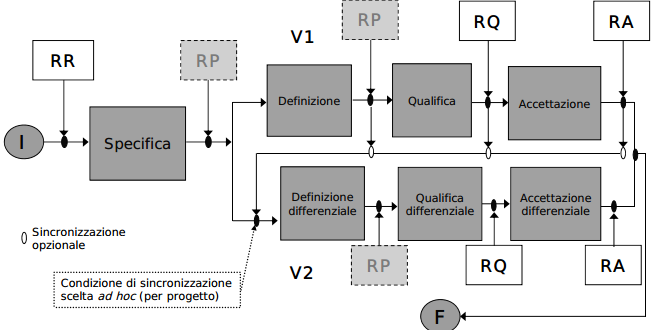
\includegraphics[width=0.5\columnwidth]{img2}

\textbf{Modello evolutivo}. E' un modello che approssima la soluzione finale ammettendo tante iterazioni, abortendo le versioni intermedie. Per poter attuare un modello evolutivo ho bisogno di tanta energia. E' una tecnica molto interessante ma con un enorme costo, infatti revisioni successive possono avere come oggetto versioni di prodotto diverse.

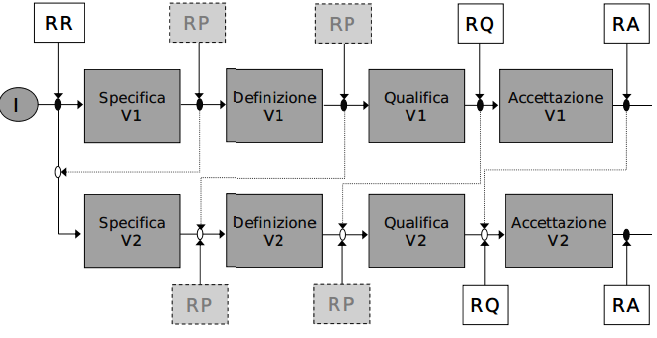
\includegraphics[width=0.4\columnwidth]{img3}
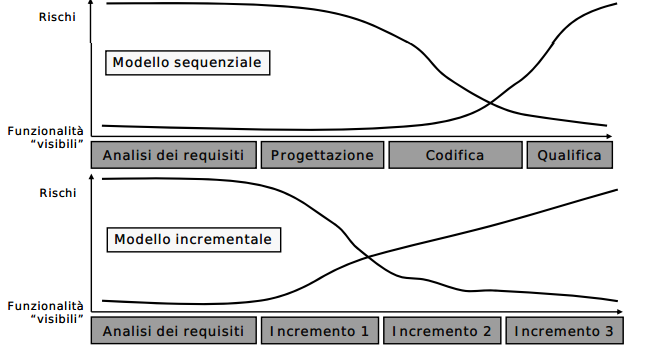
\includegraphics[width=0.4\columnwidth]{img4}

Con un modello sequenziale combatto per abbattere i rischi mandando molto avanti le funzionalità visibili, l'avanzamento infatti viene fatto solamente quando si è sicuri.\\
Con un modello incrementale riesco ad avere delle funzionalità molto prima, tuttavia ho molti più rischi possibili.

Il \textbf{modello agile} non è facilmente rappresentabile. Si ragiona sulle cose da fare (\textbf{backlog}). Fra le cose da fare in un modello agile le persone prendono liberamente quello che faranno (ciascuno pesca un post-it a seconda del proprio estro). In un modello agile l'essenziale è che per ogni cosa fatta l'effetto sia visibile (\textbf{incremental build}). Ogni aggiunta rende il prodotto sempre più vicino alle aspettative, anche se non ha un ordine particolarmente ovvio. L'unico ordine è che ci siano tante cose che posso vedere e che rappresentano ciò che il prodotto sarà . E' un modello molto interessante ma difficile da gestire.

Non tutti i problemi hanno una (buona) soluzione. Bisogna fissare con la massima chiarezza:

\begin{itemize}

	\item \textbf{Obiettivi};
	\item \textbf{Vincoli};
	\item \textbf{Alternative};
	\item \textbf{Rappresentazione del problema e delle sue soluzioni}.

\end{itemize}
la qualità cardine resta comunque \textbf{Fattibilità} e \textbf{Verificabilità}

Tecniche progettuali:
\begin{itemize}
	\item \textbf{Decomporre} in modo modulare e senza dipendenze. Una buona decomposizione identifica componenti tra loro indipendenti (a basso accoppiamento e funzionalmente coesi). La seconda cosa che voglio fare è nascondere il dettaglio implementativo (\textbf{incapsulamento}).
	\item\textbf{Accoppiamento:} è la misura dell'intensità della relazione tra parti distinte.
	\item\textbf{Coesione:} è la misura dell'intensità della relazione all'interno di una singola parte.
	\item\textbf{Astrazione:} omettere informazione per poter applicare operazioni simili ad entità diverse. Non importa la forma esatta che ha una cosa ma che abbia informazioni e funzionalità  utili, non voglio sapere tutto, ma le cose importanti in un determinato contesto.
	\item\textbf{Atomicità:} è un altro criterio molto importante. L'utilità  dell'astrazione non migliora se divido ulteriormente, perché scomporre più del dovuto ha un costo.
\end{itemize}

\textbf{Concorrenza:} è molto importante garantire al sistema una concorrenza, ma va ben gestita e se la uso in modo inconsapevole faccio solo danni.
\textbf{Distribuzione:} se e come i componenti sono disseminati su più nodi di elaborazione e come comunicano tra di loro.


Un problema grosso nella produzione del codice è che non siamo in generale preparati ad avere una buona strategia di \textbf{gestione degli errori}:

\begin{itemize}
	\item \textbf{Relativi al flusso di dati:} non posso assumere che l'utente inserisca sempre dati corretti, ma allo stesso tempo non posso accettare \textit{spazzatura}. Sugli input non posso fare assunzioni ottimistiche. Problematiche relative alla disponibilità di un dato.
	\item \textbf{Relativo al flusso di controllo:} le azioni che avvengono, gestione di eccezioni che io sollevo o che il sistema genera. Le eccezioni sono problemi che rendono il flusso di controllo instabile, e devo avere una strategia di gestione, altrimenti possono essere dannose.
	\item \textbf{Relative al trascorrere del tempo:} ci possono essere degli impegni che il programma si è preso nei confronti dell'utente (es. mi aspetto che il programma risponda in tot secondi). Devo mettere quindi un limite rispetto al quale mi aspetto qualcosa. L'utente si immagina che il sistema garantisca delle funzionalità in un tempo finito.
\end{itemize}

Si può fare progettazione parallela solo se ho costruito un'architettura progettuale che garantisca il disaccoppiamento. Devo garantire l'integrità concettuale, desiderabile in ogni architettura di sistema. Il raccordo tra programmazione e progettazione deve essere esplicito, ci deve essere coerenza. \textbf{Enforce intentions:} l'atto di assicurarsi conformità, "fai in modo che il codice realizzi precisamente le indicazioni della progettazione". Ciò che dico nell'architettura deve essere vero nel codice. La programmazione non deve fare scelte libere, ma rispettare la progettazione. La \textbf{programmazione difensiva}, essere esplicitamente pronti a trattare errori, si fa in due modi:

\begin{itemize}

	\item \textbf{Incapsulamento degli errori:} in tutti i luoghi del codice dove so che posso non avere successo devo poter gestire l'errore. Programmare esplicitamente il trattamento dei possibili errori, \textbf{errori dei dati in ingresso} ed errori logici;
	\item La strategia di trattamento va prevista nella progettazione.

\end{itemize}
Possiamo gestire due tipi di errori in diversi modi:
\begin{itemize}

	\item \textbf{Errori Dati:}

	\begin{itemize}

		\item Attendere fino all'arrivo di un valore legale;
		\item Assegnare un valore predefinito (\textit{default});
		\item Usare un valore precedente;
		\item Registrare l'errore in un \textit{log}, per avere un registro di manutenzione;
		\item Sollevare eccezioni (se ho un gestore delle eccezioni);
		\item Abbandonare il programma (se proprio non ce la faccio).

	\end{itemize}
	
	\item \textbf{Errori Logici:}


	\begin{itemize}

		\item \textbf{Aritmetica in virgola mobile:} la sua approssimazione può cumularsi e condurre a errori importanti e a confronti svianti. Essa è intrisecamente imprecisa, sono operazioni spesso fonti di errore;
		\item \textbf{Puntatori e limiti delle strutture}, i puntatori sono in generale molto pericolosi. Nel momento in cui manipolo indirizzi porto cose ovunque (\textit{segmentation fault}). Devo avere una programmazione che mi garantisca che queste cose non accadano. Voglio imporre che ai dati ci si acceda attraverso \textit{metodi di interfaccia};
		\item \textbf{Allocazione dinamica della memoria}, può portare a esaurimento della disponibilità e alla sovrapposizione di aree sensibili (il garbage collector arriva di tanto in tanto...). CHi fa un programma deve sapere quante \textit{new} può fare (oppure non le fa);
		\item \textbf{Ricorsione}, può portare all'esaurimento della memoria o alla non terminazione. La ricorsione in ogni applicativo ragionevolmente serio è un concetto \textbf{proibito}, consuma lo stack. La combinazione di \textit{new} e ricorsione è ancora peggio;
		\item \textbf{Concorrenza}, se mal progettata può condurre a errori.

	\end{itemize}
\end{itemize}


\end{document}